\chapter{Literature Survey}
This survey has been broken down into two main sections: Dynamic Similarity which will detail current research performed by \cite{Alexander1983} along with an explanation on potential shortcoming of the research and Gait Generation, which will explain in more detail the concept of a Central Pattern Generator before focusing on potential methods of gait generation found for this project.
\section{Dynamic Similarity}


The concept of Dynamic Similarity is mentioned in \cite{Skrba2010}, which describes potential quadruped animation methods, it is however only used as a guideline for animators to follow. Additionally, \cite{Skrba2010} mentions the difficulty in current methods of  gaits animation and generation. Standard motion capture is shown to be difficult with wild animals, with the data being specific to the animal trained on, making it difficult to extend on other mammals. This is seen with \cite{Alexander1983} attempting to find gait values for wild Coypu, which provide far different results to the rest of the trends seen, due to the Coypu acting in a "nervous manner". 
% Additionally, motion capture data will not be gathered for this dissertation, reducing the risk of data captured being "very specific to a particular animal and its movements"
% As this dissertation aims to use the Dynamic Similarity hypothesis as not a guideline, this should provide a more generic way of creating animal gaits. 
\cite{Alexander1983}contains a large amount of information on how the Froude number is shown to affect separate parts of mammals, as graph data is shown for Phase Relationships, Relative Stride Lengths and Forces on The Feet. 

This leads to the assumption that given the height of the animal as well as a Froude Number to represent gait, the speed of a certain gait can therefore be inferred. Dynamic Similarity is most apparent in Cursorial Mammals, which  exhibit similar relative stride lengths at the same Froude Numbers Equations for stride length against Froude number have been found in Alexander's research to take the following form, for walking gaits, a =, with b=, with faster gaits taking the following form. 


\cite{Alexander1983} makes an important distinction between non-cursorial and cursorial mammals with the hypothesis remaining accurate for examining only cursorial or non-cursorial mammals, but becoming inaccurate when considering both. Cursorial Mammals are typically referred to as animals that have adapted to run, although \cite{Garland1993} states that this not a strong enough metric for whether a mammal is cursorial. \cite{Stein1997} defines cursorial mammals as having limbs in the parasaggital plane. The saggital plane divides the body into two halves vertically, with the parasaggital plane referring to anywhere parallel to this plane. A visual example of the parasaggital plane in a cursorial mammal can be seen in \ref{fig:parasaggital}. 
 
\begin{figure}
    \centering
    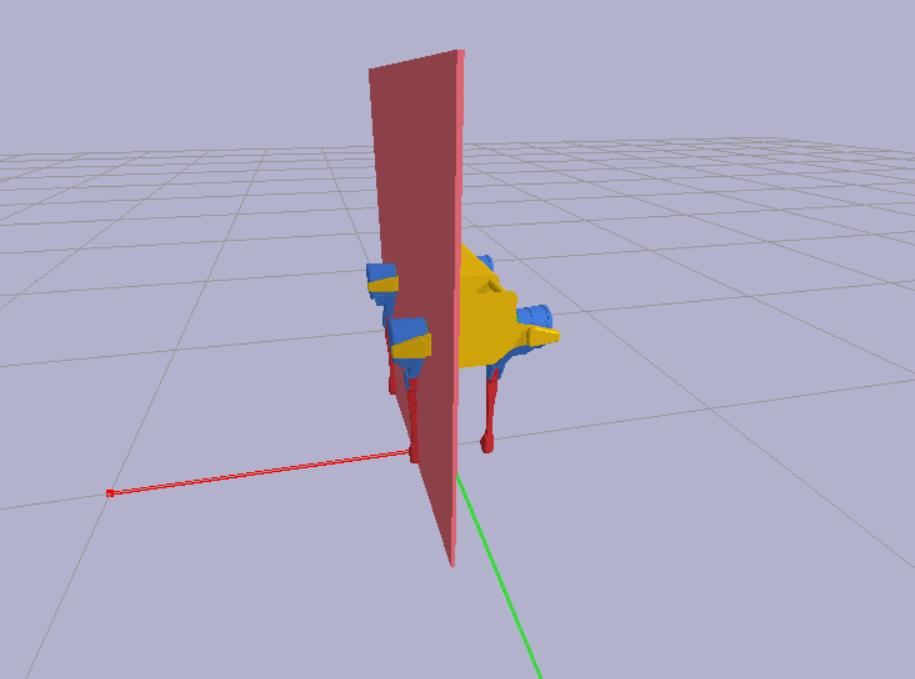
\includegraphics[width=0.4\textwidth]{figures/parasaggital.png}
    \caption{Diagram of robot parasaggital plane, indicated by the red square}
    \label{fig:parasaggital}
\end{figure}

The difference in Dynamic Similarity between cursorial and non-cursorial mammals is thought to be due to non-cursorial mammals having a far longer relative stride length than cursorial mammals. \cite{Gan2018a} investigates Dynamic Similarity between bipeds and quadrupeds, which further showcase the limitations of this Hypothesis, as there only exists similarity between quadrupeds and bipeds in  specific scenarios such as bounding. This in turn limits the Dynamic Similarity Hypothesis to cursorial mammals.


In order to showcase similarity between cursorial gaits \cite{Alexander1983} defined two separate subsets: walking, which occurs at Froude numbers below 0.4 and faster gaits, which occur above 0.4. Animals performing gaits have been described the equation \ref{froude:equation}, with x representing values of relative stride lengths. \cite{Carr2016} defines Stride Length as the distance from one step to the next step of the same leg. 

\begin{equation}
x = a*(v^2/gh)^b
\label{froude:equation}
\end{equation}

Parameter a, exponent b, deviations and froude number limits are defined by table \ref{table:froude}. As this data was gathered in 1983, the testing methods have a large margin of error.

\begin{table}[width=15cm]
\begin{tabular}{lllll}
Gait         & Factor a & Exponent b   & Standard Deviation & Froude Number Limits \\
Cursorial Walking      & 2.4      & 0.34 +- 0.1  & 1.16                      & F \textless 0.4       \\
Cursorial Faster Gaits & 1.9      & 0.40 +- 0.03 & 1.14                      & F \textgreater 0.4    \\
                               &          &              &                           &                      
\end{tabular}
\caption{Table of Froude number values}
\label{table:froude}
\end{table}

A similar concept to Dynamic Similarity although not specific to Animal Locomotion has been developed by \citep{Reveret2009} who uses expert animators in order to create morph-able quadruped skeletons. As a large amount of data is based on animator design, it may not be scientifically suitable, but it does show the potential of creating adaptable mammalian quadruped skeletons, and as the skeleton allows for morphing based on geometric measurements, a similar method could be used in order to build a robotic model. 

\section{Gait Generation}

A Central Pattern Generator is a biological neural network that provides an animal with it's natural walking rhythm, however it is also used in other actions that require periodic movements, such as chewing and breathing.  \cite{MarderEveBucher2001} shows how central pattern generators work in living mammals by investigating the movement of a locust's wings. This in turn finds that the mechanisms of rhythm generation are created by the use of neurons that produce periodic signals to couple, and produce more complex rhythmic patterns, such as walking. There are various methods for the recreation of Central Pattern Generators. 

\citep{Kruger2014} provides multiple methods of gait reconstruction, and evaluates their success rate. Although focused on retrieval from motion capture data, which is not the primary focus of this project, it highlights the primary issues with gathering motion capture data and using it to infer gaits, as although the experiments shown in \cite{Kruger2014} are successful, there does not exist a large motion capture database. This correlates with information gathered from \cite{Skrba2010}, which claims that the major issue with gathering motion capture data is that wild animals are difficult to gather a large dataset for.

\cite{Geijtenbeek2013} produces a method of locomotion for different types of bipeds through the implementation of a musco-skeletal model. Although this sort of model would not be possible to directly be implemented into a robotic design due to the high complexity of the model, and it does not involve a neuronal central pattern generator (instead using a finite state machine to decide method constriction and expansion), it showcases the possibility of a locomotion system being adaptable to multiple models. One of the methods that \cite{Geijtenbeek2013} uses in order to optimise the gaits is through the use of a Covariance Matrix Adaptation \cite{Hansen2016}, an evolutionary principle that is particularly effective in small population sizes, and so would be effective in the small populations used in \cite{Geijtenbeek2013}. 

An interesting implementation of recreating quadruped gaits is shown in \cite{Zhang2018}, who proposes using Mode-Adaptive Neural Networks. It is used to create a variety of complex movements such as obstacle navigation, jumping and gait correction. The focus of \cite{Zhang2018} was in creating realistic animations, and as they are not applied directly to the design of a robot, the methods seen may not apply to a real model of a robot. Additionally, \cite{Zhang2018} gathers data based from Dog motion capture data, which means that the design of the network is focused on data from dog gaits, and would be unable to easily translate to other animals. 

\cite{Fukuoka2015} implements gait generation  through the use of a CPG and applies leg loading feedback to assist in navigation of uneven surfaces. This design applies to normal gaits as well as converting between walking and faster gaits. The design of this 

A frequently used method has been through the use of non-conservative oscillators. \cite{Rutishauser2008} implements a central pattern generator through the use of a derivative equation, with oscillators being coupled together through the use of a 4x4 size matrix. This produces a stable walking gait, however comes into trouble when trying to replicate a faster gait pace. However, \cite{Rutishauser2008} appears to find a walking gait far more stable than that of a trot, with a trot performing far less stable and slower gaits, and actually being far more unstable at faster speeds. 

Van der Pol oscillators have shown to be extremely common in the replication of central pattern generators, being used successfully in \cite{Low2006} for the replication of Jellyfish Locomotion. A Van der Pol Oscillator is a non-linear oscillator that can be described by a second-order differential equation \citep{Barbosa2007}. The equation of a normal Van der Pol oscillator is described by equation \ref{vanderpol:pure}
\begin{equation}
\ddot{x} + \alpha(x^2 - 1)\dot{x} + x = 0
\label{vanderpol:pure}
\end{equation}

\cite{Collins1994} investigates multiple different non-linear oscillators for the replication of quadruped gaits, one of the types of non-linear oscillators that stands out is the Van der Pol oscillator. \cite{Collins1994} used coupled Van der Pol generators to recreate quadruped gaits mathematically. Although this is not implemented in a real model, it appears to shows how the generator can create transitions from different gaits, and react to real-time changes in coupling parameters. The slightly modified Van der Pol oscillator in \cite{Collins1994} is described by equation \ref{vanderpol:mod}.

\begin{equation}
\ddot{x} + \mu(x^2 - p^2)\dot{x} + g^2x = 0
\label{vanderpol:mod}
\end{equation}

Where mu, p and g are free parameters. This allows more direct control over the period and shape of the Van der Pol oscillator.

\cite{Yocono2015} describes the dynamics of a van der pol oscillator in more detail, and provides an implementation of a Van der Pol oscillator in python, showcasing the use of the oscillator in hair cell auditory responses. However, \cite{Yocono2015} does not implement coupling of any form for this. \cite{Yocono2015} uses a modified Van der Pol oscillator as seen in equation \ref{vanderpol:mod}, which suggests that this modified form is common.

\cite{Liu2009} provides an implementation of a Van der Pol oscillator in a robotic quadruped. For this implementation, $x^2$ and $p^2$ are switched around, and the equation is put into a two-dimensional form for ease of implementation. This results in \ref{vanderpol:twod} 


\begin{equation}
\dot{x} = y,   \dot{y} = \alpha(p^2 - x^2)y - w^2x
\label{vanderpol:twod}
\end{equation}

This equation is shown to produce valid walking, trotting, bounding and pacing gaits. However, only the success of the implementation is measured, with no work done on improving efficiency or energy expenditure. Additionally, the parameters used for this paper are arbitrary. \cite{Liu2019} shows that implementation of a van Der Pol oscillator into a robot quadruped can produce successful gaits and do it through the use of a relatively simple differential equation. Coupling in \cite{Liu2009} is performed in a similar way to the coupling found in \cite{Collins1994}. This is done through the use of a 4x4 matrix of values, with a coupling parameter for each limb, with the equation for coupling oscillator a to oscillator i can be seen in equation \ref{vanderpol:coupling}

\begin{equation}
x_{ai} = x_{i} + \sum_{j}{\lambda_{ij}x_{j}}
\label{vanderpol:coupling}
\end{equation}

Due to the similarity between the coupling found in \cite{Collins1994} and \cite{Liu2009}, this appears to be a common method of coupling between oscillators. One of the interesting differences is that although both oscillator equations are almost identical, the coupling matrices for \cite{Collins1994} and \cite{Liu2009} are different. This could be due to different parameters used in \cite{Collins1994} due to them not having an actual implementation in a working robot.
% balancing\citep{Meng2015}
A potential issue in gait generation for a quadruped robot is stability. \cite{Meng2015} provides a method of balancing through the use of.  \cite{PrescottTonyJLeporaNathanFVerschure2018}, which shows how the centre of mass is guided via gravity during a horse trot. By following optimal speeds at certain gaits, this could potentially to allow the Centre Of Mass of the system to 'float' when encountered with small obstacles, essentially dealing with small issues

% \citep{PrescottTonyJLeporaNathanFVerschure2018}
% By adhering to the evolutionary principle, this could provide a method in which some natural stability might be observed. This can be seen in
% \begin{equation}
% \ddot{x} + \alpha(x^2 - 1)\dot{x} + x = 0
% \label{vanderpol:pure}
% \end{equation}

% \begin{equation}
% \ddot{x} + \alpha(x^2 - 1)\dot{x} + x = 0
% \label{vanderpol:pure}
% \end{equation}


% \begin{equation}
% \ddot{x} + \alpha(x^2 - 1)\dot{x} + x = 0
% \label{vanderpol:pure}
% \end{equation}

% \begin{equation}
% M = \frac{1}{T}\sum_{t=1}^{T} e(t) / \max_{t}[e(t)]
% \label{eq:equation}
% \end{equation}

%   % Replace with your text

% This is shown in Equation \ref{eq:equation} and is repeated here $M = \frac{1}{T}\sum_{t=1}^{T} e(t) / \max_{t}[e(t)]$.


% \section{Evaluation}

% \begin{figure}[ht]
% 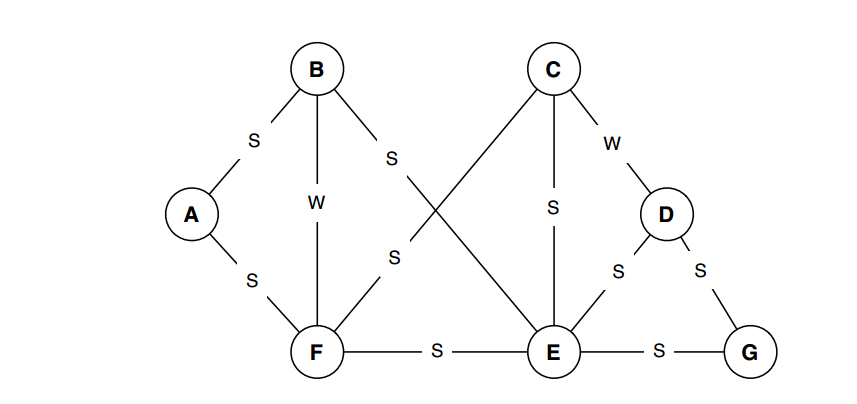
\includegraphics[width=15cm]{figures/figure1.png}
% \caption{A simple figure in \LaTeX. Reproduced from http://tinyurl.com/nqtrlj5 with the permission of the copyright owner.}
% \label{fig:graph}
% \end{figure}

  % Replace with your text

% See Figure \ref{fig:graph}.


  % Replace with your text

% \begin{table}[ht]
% \center
% \begin{tabular}{cc|c}
% A & B & A XOR B\\
% \hline
% 0 & 0 & 0\\
% 0 & 1 & 1\\
% 1 & 0 & 1\\
% 1 & 1 & 3\\
% \end{tabular}
% \caption{A simple table in \LaTeX.}
% \label{tab:xor}
% \end{table}

  % Replace with your text

% This is shown in Table \ref{tab:xor}.


\section{Summary}
Through this review, many valid methods where found for the recreation of a living mammals Central Pattern Generator. However, very few of the current methods seen use the concept of Dynamic Similarity to a large extent.

The research found in \cite{Alexander1983} is slightly out-dated, especially with the methods of data collection, such as the use of extrapolation over distance for certain African mammals. However, this does not make the hypothesis invalid, as it has shown to apply for a wide range of animals tested.

Although there are a wide range of methods for creating Central Pattern Generators, many use methods that would not be directly applicable to a real robot, such as the recreation of muscular skeletal systems in \cite{Geijtenbeek2013} or would be outside the scope of the Dissertation. The use of coupled non-linear oscillators, due to it's relative simplicity as well as effectiveness in generating robotic gaits seems to be appropriate in scope, and would be able to produce valid gaits.

Although various models have been investigated on how to generate realistic quadruped gaits, a model has not been found that compares against results found in Dynamic Similarity. This could be especially useful for the Van der Pol oscillator due to it's effectiveness in modelling other natural systems.

% \begin{figure}
%     \centering
%     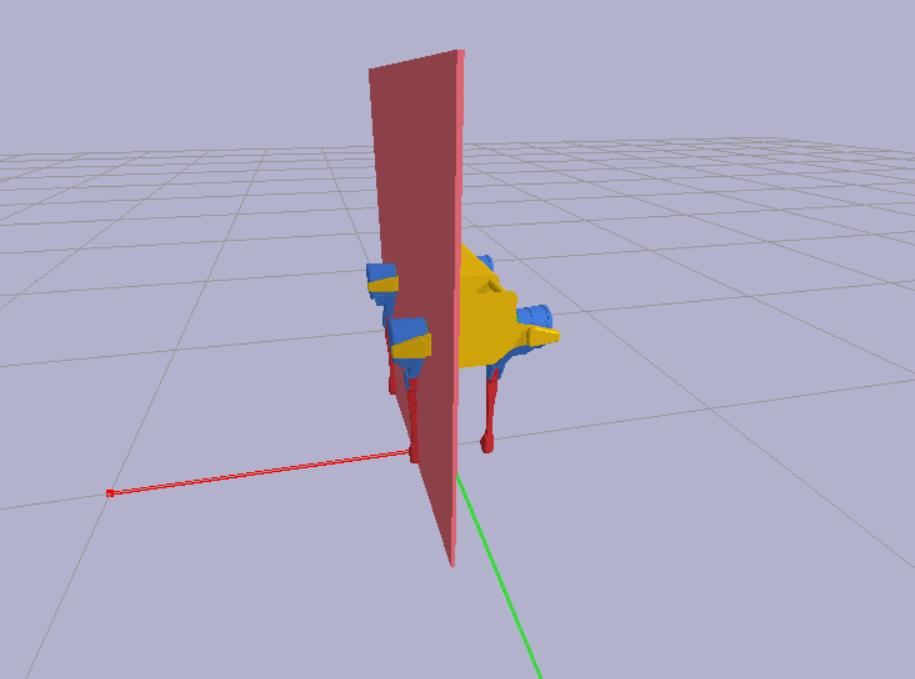
\includegraphics[width=0.8\textwidth]{figures/parasaggital.png}
%     \caption{Diagram of robot planes, the red square indicates the robots Parasaggital plane.}
%     \label{fig:vanderpol}
% \end{figure}

% There are many different available options of oscillator, from the Stein neuronal model, which is typically used to simulate a neuron itself. In this paper, we wish to focus on the investigation of the van der pol oscillator, which takes the following second-order nonlinear differential equation, this equation can be seen in \ref{vanderpol:pure}.


% Certain gaits can be shown mathematically, for example, \cite{} describes the following gaits numerically, with phase difference between gaits being labelled. 
% \begin{figure}
%     \centering
%     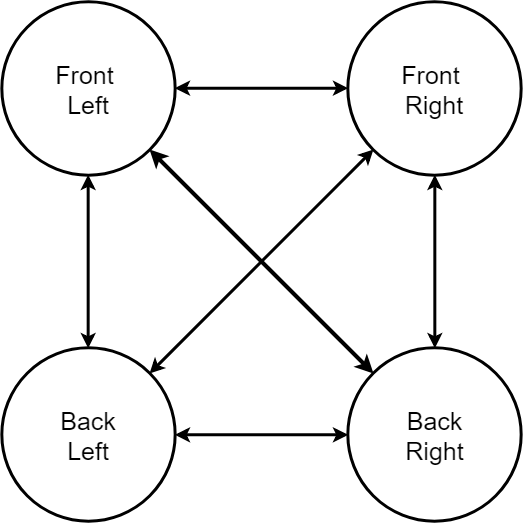
\includegraphics[width=0.3\textwidth]{figures/coupling.png}
%     \caption{Diagram of coupling combinations.}
%     \label{fig:coupling}
% \end{figure}
